\documentclass[12pt]{article}
\usepackage{times}
\usepackage{amsmath}
\usepackage{amssymb}
\usepackage[pdftex]{graphicx} % Need this for MAC, comment out for PC
\usepackage{epstopdf}         % Need this for MAC, comment out for PC
%\usepackage{epsfig}           % Need this for PC, comment out for MAC
\usepackage{ITC}

\usepackage{ifpdf}
\ifpdf
\usepackage[pdftex]{graphicx} % Use this for the Mac
\usepackage{epstopdf}         % Use this for the Mac
\else
\usepackage{graphicx}         % Use this for the PC
\fi

\title{\Large \vspace{-0.5in}
\MakeUppercase{Title of Paper in All Capital Letters}}
\author{Author(s) Name(s)\\
    \normalsize Affiliation 1 (Department, Division, etc.)\\
    \normalsize Affiliation 2 (Company, Agency, University, etc.)\\
    \normalsize City, ST, ZIP (add additional lines as needed\\
    \normalsize email@domain.com\\[6pt]
    [For student papers] Faculty Advisor: \\
    Name of Advisor}

\date{}

\begin{document}

\maketitle %\thispagestyle{empty} \pagestyle{empty}





\section{\MakeUppercase{Abstract}}

\noindent
The abstract is a brief summary of the paper, outlining the key problem addressed, methodology, and main findings. It should be no longer than 200 words and provide a clear overview of the paper’s purpose.



\section{\MakeUppercase{Introduction}}

\noindent
The Introduction introduces readers to the paper. It should provide background information, the motivation for the paper, its objectives, and a brief outline of the main sections.



\section{\MakeUppercase{The Body}}
\label{sec:Body}

\noindent
This section should be structured into multiple subsections as needed. It typically includes explanations, equations, figures, and tables. ITC technical papers have a {\bf 15-page limit}. With LaTeX, the template formats a lot of things for you, and so we will just include a few representative examples of equations/figures/etc.



\section{\MakeUppercase{Citations and Other References}}
\label{sec:Body}

\noindent

Here are some citations of a single item~\cite{CcsdsOrangeBook} and multiple items~\cite{ChalfantIrving,CoverBook,DapperHill,ForneyVa,Irig106-04,LiSimon}, notice that these include examples of conference papers, journal papers, etc. The numbers you see above are AUTOMATICALLY UPDATED when you add/remove/rearrange the list of references at the end of the paper.

~\\
\noindent
Here is an example of an equation
\begin{equation}
E = mc^2.
\label{eq:EnergyMass}
\end{equation}
That equation ended its sentence, so it has a period at the end. We can reference~\eqref{eq:EnergyMass} by using its number.

An example figure is shown in Figure~\ref{fig:Downsample}, where we again reference something using its number.

\begin{figure}
\centering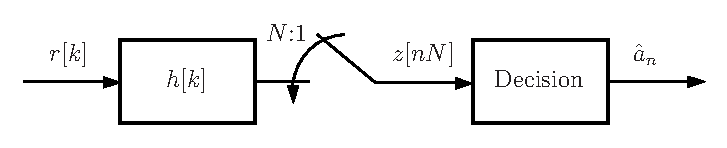
\includegraphics[width=3.75in]{figures/Downsample}
\caption{Downsampling operation.}
\label{fig:Downsample}
\end{figure}




\section{\MakeUppercase{Numerical Results}}
\label{sec:NumericalResults}

\noindent
If applicable, present numerical results, performance analysis, or experimental data.



\section{\MakeUppercase{Conclusions}}
\label{sec:Conclusions}

\noindent
In this section, summarize the key findings of your paper, their implications, and potential areas for future research. Reinforce the significance of your work by highlighting its impact and benefits to the reader. Consider connecting your results to a broader context, discussing their relevance, and revisiting your paper’s central question with the new insights you have presented.



\bibliographystyle{ieeetr}
\bibliography{references}
\end{document}
